\section{Auswertung}
\label{sec:Auswertung}
\subsection{Zeitabhänigkeit der Amplitude einer gedämpften Schwingung}
  Zuerst werden alle Werte logarithmiert und die Werte der
  oberen und unteren Einhüllenden werden dann mit der Funktion
  \begin{equation*}
    f(x)= 2\pi\mu t + \symup{ln} (A_0)
  \end{equation*}
  gefittet, wie in Abbildung \ref{fig:5aplot} zusehen.
    \begin{figure}
      \centering
      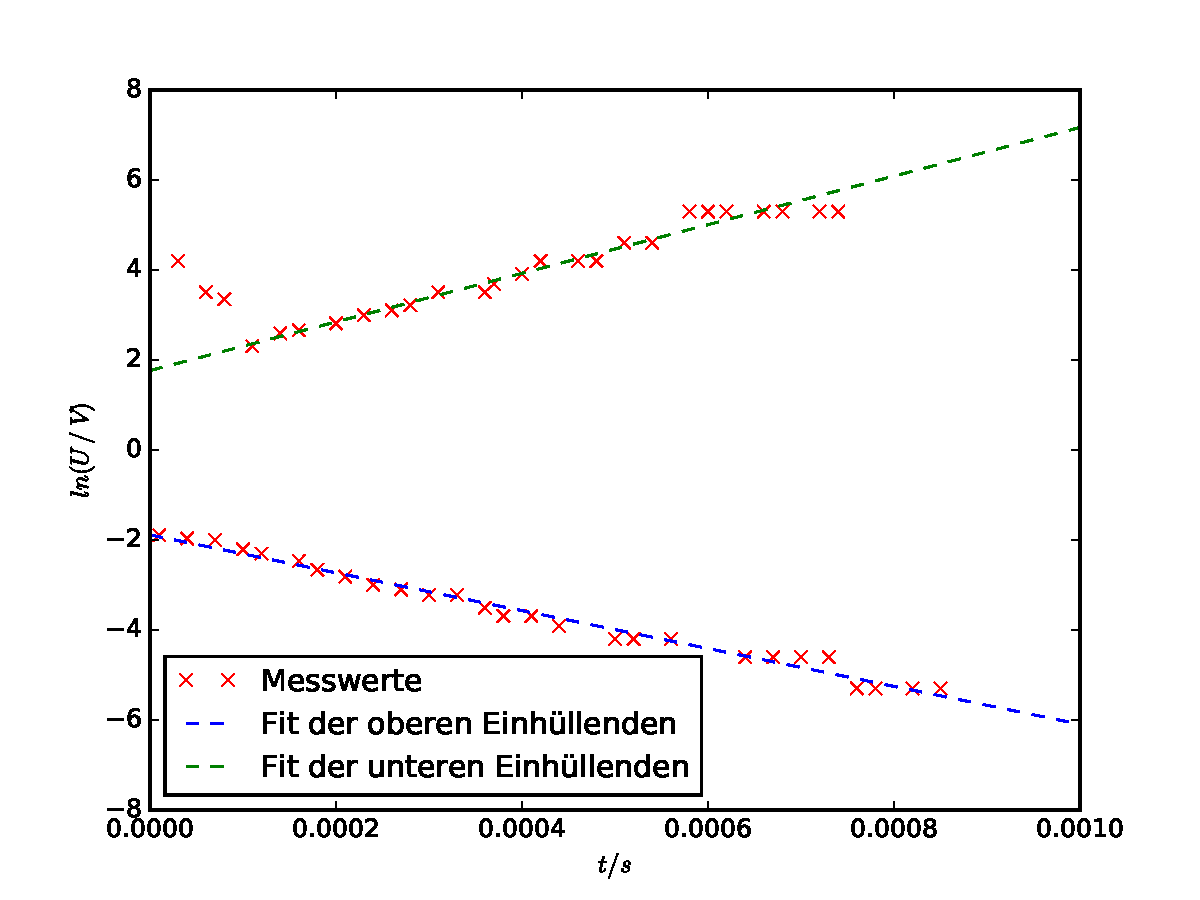
\includegraphics[width=\textwidth]{./plots/5aplotreload.pdf}
        \caption{Einhüllenden der Schwingungskurve}
        \label{fig:5aplot}
      \end{figure}
\FloatBarrier
Es ist ersichtlich, dass für den Fit der unteren Einhüllenden,
Werte aus gelassen wurden, da
diese keine Aussage über den Abfall der Schwingung machen,
 sonder Ergebniss des Anschwingvorganges sind.
  Aus dem Fit ergebn sich dann folgende Werte für die obere Einhüllende
  \begin{equation*}
    \mu = (-670 \pm 17)\; \frac{1}{\symup{s}}
    \qquad A_0  = (0,152 \pm 0,008) \;\symup{V}
  \end{equation*}
  und für die untere Einhüllende
  \begin{equation*}
    \mu = (860 \pm 34) \; \frac{1}{\symup{s}}
     \qquad A_0 = (5,8 \pm 0,6)\;\symup{V}.
  \end{equation*}
  Daraus ergeben sich dann Werte für die Abklingdauer
  \begin{equation*}
    T_{ex} = \frac{1}{2\pi\mu}
  \end{equation*}
  und dem effektiv Widerstand
  \begin{equation*}
    R_{eff} = 4\pi L \mu.
  \end{equation*}
Daraus ergeben sich dann die Werte
\begin{equation*}
  T_{ex}=(2,38\cdot 10^{-5} \pm 6\cdot 10 ^{-6})\; \symup{s} \; \text{und} \;
  R_{eff} = (85,1 \pm 2,2) \;\symup{\Omega}
\end{equation*}
für die obere Einhüllende und
\begin{equation*}
  T_{ex}=(1,85\cdot 10^{-5} \pm 7\cdot 10 ^{-6})\; \symup{s} \; \text{und} \;
  R_{eff} = (109 \pm 4) \;\symup{\Omega}
\end{equation*}
für die untere Einhüllende. Die Werte von diesem Teil des Versuches sind in den
folgenden Tabellen eingetragen.
  \begin{table}
    \caption{Spannung und Frequenz der Gedämpften Schwinung}
  \begin{subfigure}{0.48\textwidth}
  \caption{1}
  \label{tab:5a1tab}
  \sisetup{round-mode = places , round-precision = 2}
  \begin{tabular}{S S}
    \toprule
    {$U_i/\symup{mV}$} & {$t/\symup{\mu s}$ }\\
    \midrule
    1.500000000000000000e+02 & 1.000000000000000000e+01\\
    1.400000000000000000e+02 & 4.000000000000000000e+01\\
    1.350000000000000000e+02 & 7.000000000000000000e+01\\
    1.100000000000000000e+02 & 1.000000000000000000e+02\\
    1.000000000000000000e+02 & 1.200000000000000000e+02\\
8.500000000000000000e+01 & 1.600000000000000000e+02\\
7.000000000000000000e+01 & 1.800000000000000000e+02\\
6.000000000000000000e+01 & 2.100000000000000000e+02\\
5.000000000000000000e+01 & 2.400000000000000000e+02\\
4.500000000000000000e+01 & 2.700000000000000000e+02\\
4.000000000000000000e+01 & 3.000000000000000000e+02\\
4.000000000000000000e+01 & 3.300000000000000000e+02\\
3.000000000000000000e+01 & 3.600000000000000000e+02\\
2.500000000000000000e+01 & 3.800000000000000000e+02\\
2.500000000000000000e+01 & 4.100000000000000000e+02\\
2.000000000000000000e+01 & 4.400000000000000000e+02\\
1.500000000000000000e+01 & 5.000000000000000000e+02\\
1.500000000000000000e+01 & 5.200000000000000000e+02\\
1.500000000000000000e+01 & 5.600000000000000000e+02\\
1.000000000000000000e+01 & 6.400000000000000000e+02\\
1.000000000000000000e+01 & 6.700000000000000000e+02\\
1.000000000000000000e+01 & 7.000000000000000000e+02\\
1.000000000000000000e+01 & 7.300000000000000000e+02\\
5.000000000000000000e+00 & 7.600000000000000000e+02\\
5.000000000000000000e+00 & 7.800000000000000000e+02\\
5.000000000000000000e+00 & 8.200000000000000000e+02\\
5.000000000000000000e+00 & 8.500000000000000000e+02\\
1.500000000000000000e+01 & 3.000000000000000000e+01\\
3.000000000000000000e+01 & 6.000000000000000000e+01\\
3.500000000000000000e+01 & 8.000000000000000000e+01\\
-1.000000000000000000e+02 & 1.100000000000000000e+02\\
-7.500000000000000000e+01 & 1.400000000000000000e+02\\
-7.000000000000000000e+01 & 1.600000000000000000e+02\\
-6.000000000000000000e+01 & 2.000000000000000000e+02\\
-5.000000000000000000e+01 & 2.300000000000000000e+02\\
-4.500000000000000000e+01 & 2.600000000000000000e+02\\
-4.000000000000000000e+01 & 2.800000000000000000e+02\\
-3.000000000000000000e+01 & 3.100000000000000000e+02\\
-3.000000000000000000e+01 & 3.600000000000000000e+02\\
-2.500000000000000000e+01 & 3.700000000000000000e+02\\
\bottomrule
\end{tabular}
\end{subfigure}
\begin{subfigure}{0.48\textwidth}
\caption{2}
\label{tab:5a2tab}
\sisetup{round-mode = places , round-precision = 2}
\begin{tabular}{S S}
\toprule
{$U_i/\symup{mV}$} & {$t/\symup{\mu s}$ }\\
\midrule
-2.000000000000000000e+01 & 4.000000000000000000e+02\\
-1.500000000000000000e+01 & 4.200000000000000000e+02\\
-1.500000000000000000e+01 & 4.600000000000000000e+02\\
-1.500000000000000000e+01 & 4.800000000000000000e+02\\
-1.000000000000000000e+01 & 5.100000000000000000e+02\\
-1.000000000000000000e+01 & 5.400000000000000000e+02\\
-5.000000000000000000e+00 & 5.800000000000000000e+02\\
-5.000000000000000000e+00 & 6.000000000000000000e+02\\
-5.000000000000000000e+00 & 6.200000000000000000e+02\\
-5.000000000000000000e+00 & 6.600000000000000000e+02\\
4.000000000000000000e+01 & 3.000000000000000000e+02\\
4.000000000000000000e+01 & 3.300000000000000000e+02\\
3.000000000000000000e+01 & 3.600000000000000000e+02\\
2.500000000000000000e+01 & 3.800000000000000000e+02\\
2.500000000000000000e+01 & 4.100000000000000000e+02\\
2.000000000000000000e+01 & 4.400000000000000000e+02\\
1.500000000000000000e+01 & 5.000000000000000000e+02\\
1.500000000000000000e+01 & 5.200000000000000000e+02\\
1.500000000000000000e+01 & 5.600000000000000000e+02\\
1.000000000000000000e+01 & 6.400000000000000000e+02\\
1.000000000000000000e+01 & 6.700000000000000000e+02\\
1.000000000000000000e+01 & 7.000000000000000000e+02\\
1.000000000000000000e+01 & 7.300000000000000000e+02\\
5.000000000000000000e+00 & 7.600000000000000000e+02\\
5.000000000000000000e+00 & 7.800000000000000000e+02\\
5.000000000000000000e+00 & 8.200000000000000000e+02\\
5.000000000000000000e+00 & 8.500000000000000000e+02\\
1.500000000000000000e+01 & 3.000000000000000000e+01\\
3.000000000000000000e+01 & 6.000000000000000000e+01\\
3.500000000000000000e+01 & 8.000000000000000000e+01\\
-1.000000000000000000e+02 & 1.100000000000000000e+02\\
-7.500000000000000000e+01 & 1.400000000000000000e+02\\
-7.000000000000000000e+01 & 1.600000000000000000e+02\\
-6.000000000000000000e+01 & 2.000000000000000000e+02\\
-5.000000000000000000e+01 & 2.300000000000000000e+02\\
-4.500000000000000000e+01 & 2.600000000000000000e+02\\
-4.000000000000000000e+01 & 2.800000000000000000e+02\\
-3.000000000000000000e+01 & 3.100000000000000000e+02\\
-3.000000000000000000e+01 & 3.600000000000000000e+02\\
-2.500000000000000000e+01 & 3.700000000000000000e+02\\

\bottomrule
\end{tabular}
\end{subfigure}
\end{table}
\begin{table}
\centering
\caption{Spannung und Frequenz der Gedämpften Schwingung 3}
\label{tab:5a3tab}
\sisetup{round-mode = places , round-precision = 2}
\begin{tabular}{S S}
\toprule
{$U_i/\symup{mV}$} & {$t/\symup{\mu s}$ }\\
\midrule
-2.000000000000000000e+01 & 4.000000000000000000e+02\\
-1.500000000000000000e+01 & 4.200000000000000000e+02\\
-1.500000000000000000e+01 & 4.600000000000000000e+02\\
-1.500000000000000000e+01 & 4.800000000000000000e+02\\
-1.000000000000000000e+01 & 5.100000000000000000e+02\\
-1.000000000000000000e+01 & 5.400000000000000000e+02\\
-5.000000000000000000e+00 & 5.800000000000000000e+02\\
-5.000000000000000000e+00 & 6.000000000000000000e+02\\
-5.000000000000000000e+00 & 6.200000000000000000e+02\\
-5.000000000000000000e+00 & 6.600000000000000000e+02\\
-5.000000000000000000e+00 & 6.800000000000000000e+02\\
-5.000000000000000000e+00 & 7.200000000000000000e+02\\
-5.000000000000000000e+00 & 7.400000000000000000e+02\\
0.000000000000000000e+00 & 7.700000000000000000e+02\\
0.000000000000000000e+00 & 8.100000000000000000e+02\\
0.000000000000000000e+00 & 8.300000000000000000e+02\\
-5.000000000000000000e+00 & 6.800000000000000000e+02\\
-5.000000000000000000e+00 & 7.200000000000000000e+02\\
-5.000000000000000000e+00 & 7.400000000000000000e+02\\
0.000000000000000000e+00 & 7.700000000000000000e+02\\
0.000000000000000000e+00 & 8.100000000000000000e+02\\
0.000000000000000000e+00 & 8.300000000000000000e+02\\
\bottomrule
\end{tabular}
\end{table}
\FloatBarrier
  \subsection{Aperodischer Grenzfall}
  \begin{figure}
    \centering
    \caption{Spannungen im Schwingkreis}
    \begin{subfigure}{0.48\textwidth}
      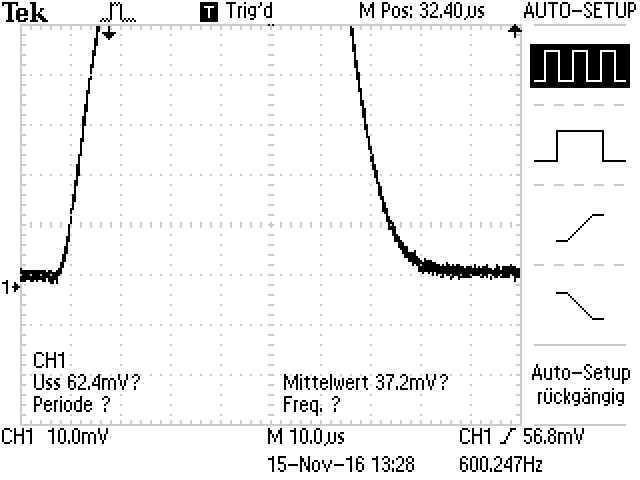
\includegraphics[height= 5cm]{./logos/5Print.JPG}
      \caption{bei einer Erregerfrequenz von 3,5 k$\symup{\Omega}$}
      \label{fig:p1}
    \end{subfigure}
    \begin{subfigure}{0.48\textwidth}
      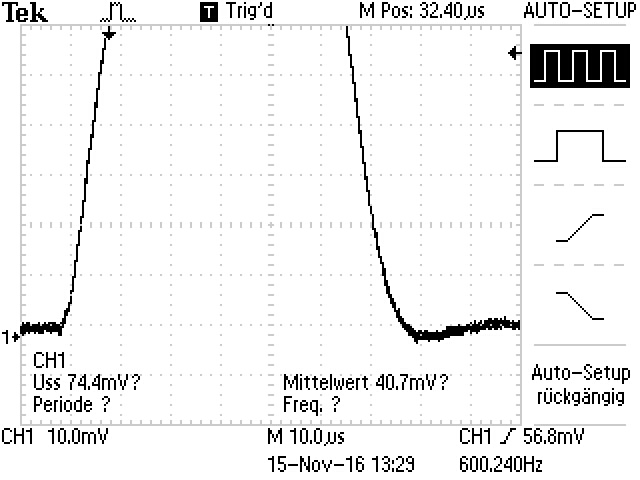
\includegraphics[height= 5cm]{./logos/6Print.JPG}
      \caption{bei einer Erregerfrequenz von 3 k$\symup{\Omega}$}
      \label{fig:p2}
    \end{subfigure}
    \\
    \begin{subfigure}{0.48\textwidth}
      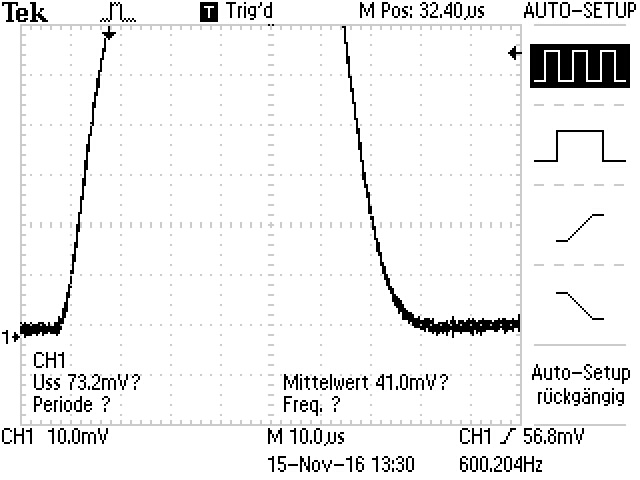
\includegraphics[height= 5cm]{./logos/7Print.JPG}
      \caption{bei einer Erregerfrequenz von 3,3 k$\symup{\Omega}$}
      \label{fig:p3}
    \end{subfigure}
      \label{fig:prints}
  \end{figure}
  \FloatBarrier
  In Abbildung \ref{fig:prints} ist zusehen, dass es einen Überschwung
  bei 3,5 k$\symup{\Omega}$

      gibt und bei 3 k$\symup{\Omega}$ die Relaxion noch nicht
      ihr Maximum erreicht hat. Daraus folgt das der Widerstand $R_{ap}$ bei ca.
      3,3 k$\symup{\Omega}$ liegt. Der Literaturwert liegt bei
      $4390 \pm 9 \;\symup{\Omega}$ .

  \subsection{Frequenzabhängigkeit der Kondensatorspannung}
  \begin{figure}
    \centering
    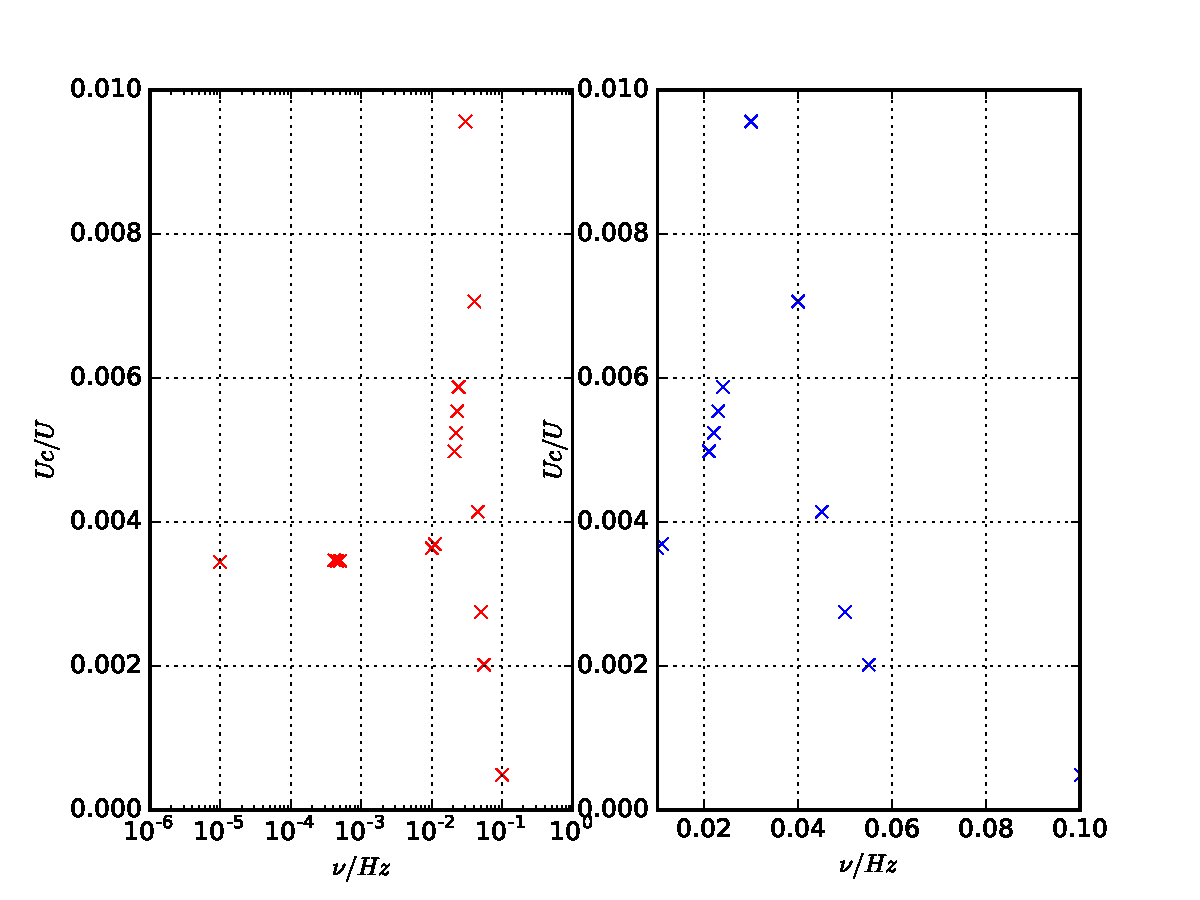
\includegraphics[height=7cm]{./plots/5cplot.pdf}
      \caption{Kondensatorspannung}
      \label{fig:5cplot}
    \end{figure}
    \FloatBarrier
    Für die Resonanzüberhöhung q ergibt sich experimentel: $q_{ex}= 2,34 $.
    Theoretisch ergibt sich jedoch : $q_{theo}= (21,8  \pm 0,5) $.
    Für den Frequenzenabstand ergibt sich experimentel $ \nu_+ - \nu_- = 25 \symup{kHz} $
    und theoretisch $ \nu_{theo}= (1585 \pm 33)\symup{Hz}$.
    Die Resonanzüberhöung ergibt sich aus der Formel
    \begin{equation*}
      q_{theo} = \frac{\omega_0}{\omega_+ - \omega_-}.
    \end{equation*}
    Der Frequenzabstand ergibt sich aus
    \begin{equation*}
      \nu_{theo} = \nu_+ - \nu_- = \frac{R}{2\pi L}
    \end{equation*}
    Die Messreihe wurde in der folgenden Tabelle festgehalten.
    \begin{table}
      \centering
      \caption{Spannung und Frequenzabhängigkeit der Kondensatorspannung}
      \label{tab:5ctab}
      \sisetup{round-mode = places , round-precision = 2}
    \begin{tabular}{S S S}
      \toprule
      $U_{ss}/\symup{mV}$ & $U_{eff}/\symup{mV}$ & $t/\symup{\mu s}$ \\
      \midrule
      1.560000000000000000e+02 & 5.550000000000000000e+01 & 4.150000000000000000e+02\\
      1.560000000000000000e+02 & 5.539999999999999858e+01 & 4.500000000000000000e+02\\
      1.560000000000000000e+02 & 5.539999999999999858e+01 & 5.000000000000000000e+02\\
      1.680000000000000000e+02 & 5.820000000000000284e+01 & 1.000000000000000000e+04\\
      1.720000000000000000e+02 & 5.910000000000000142e+01 & 1.100000000000000000e+04\\
      2.220000000000000000e+02 & 7.720000000000000284e+01 & 2.000000000000000000e+04\\
      2.720000000000000000e+02 & 9.400000000000000000e+01 & 2.400000000000000000e+04\\
      2.560000000000000000e+02 & 8.859999999999999432e+01 & 2.300000000000000000e+04\\
      2.440000000000000000e+02 & 8.379999999999999716e+01 & 2.200000000000000000e+04\\
      2.340000000000000000e+02 & 7.970000000000000284e+01 & 2.100000000000000000e+04\\
      4.480000000000000000e+02 & 1.530000000000000000e+02 & 3.000000000000000000e+04\\
      3.240000000000000000e+02 & 1.130000000000000000e+02 & 4.000000000000000000e+04\\
      1.960000000000000000e+02 & 6.629999999999999716e+01 & 4.500000000000000000e+04\\
      1.260000000000000000e+02 & 4.400000000000000000e+01 & 5.000000000000000000e+04\\
      9.440000000000000568e+01 & 3.229999999999999716e+01 & 5.500000000000000000e+04\\
      1.560000000000000000e+02 & 5.510000000000000142e+01 & 9.810000000000000497e+00\\
      2.139999999999999858e+01 & 7.799999999999999822e+00 & 1.002000000000000000e+05\\
      \bottomrule
    \end{tabular}
    \end{table}
    \FloatBarrier
  \subsection{Frequenzabhängigikeit der Phase zwischen Erreger-und Kondensatorspannung}
  Die Frequenzabhängigkeit der Phase zwischen Erreger-und Kondensatorspannung
   lässt sich im Plot \ref{fig:5dplot} betrachten.
  Aufgrund zu weniger Daten im intressanten Bereich
  können $\nu_+$ und $\nu_+$ , sowie $\nu_{res}$
  experimentel nicht eindeutig bestimmt werden. Laut den Messwerten
  müsste die Resonanzfrequenz bei ca. 5 Hz liegen, dass wiederspricht den
  Erwartungswerten.
  Die Erwartungswerte liegen für $\nu_{res}$ bei $(6,908 \pm 0,014)\cdot10^4 \;
  \frac{1}{\symup{s}}$
  und für $\nu_+$ sowie $\nu_-$ bei
  $(3,536 \pm 0,007)\cdot10^4\;\frac{1}{\symup{s}}$ \;und\; $(3,377 \pm 0,007)\cdot10^4
  \;\frac{1}{\symup{s}}$.
  Das ergibt sich aus den Gleichungen:
  \begin{equation*}
    \nu_{res} = \frac{1}{2\pi}\sqrt{\frac{1}{LC} - \frac{R^2 }{2L^2}}
    \quad \text{und} \quad
    \nu_{\pm} = \pm \frac{1}{2\pi} \left(\frac{R}{2L}
    + \sqrt{\frac{R^2}{4L^2} + \frac{1}{LC}}\right).
  \end{equation*}

    \begin{figure}
      \centering
      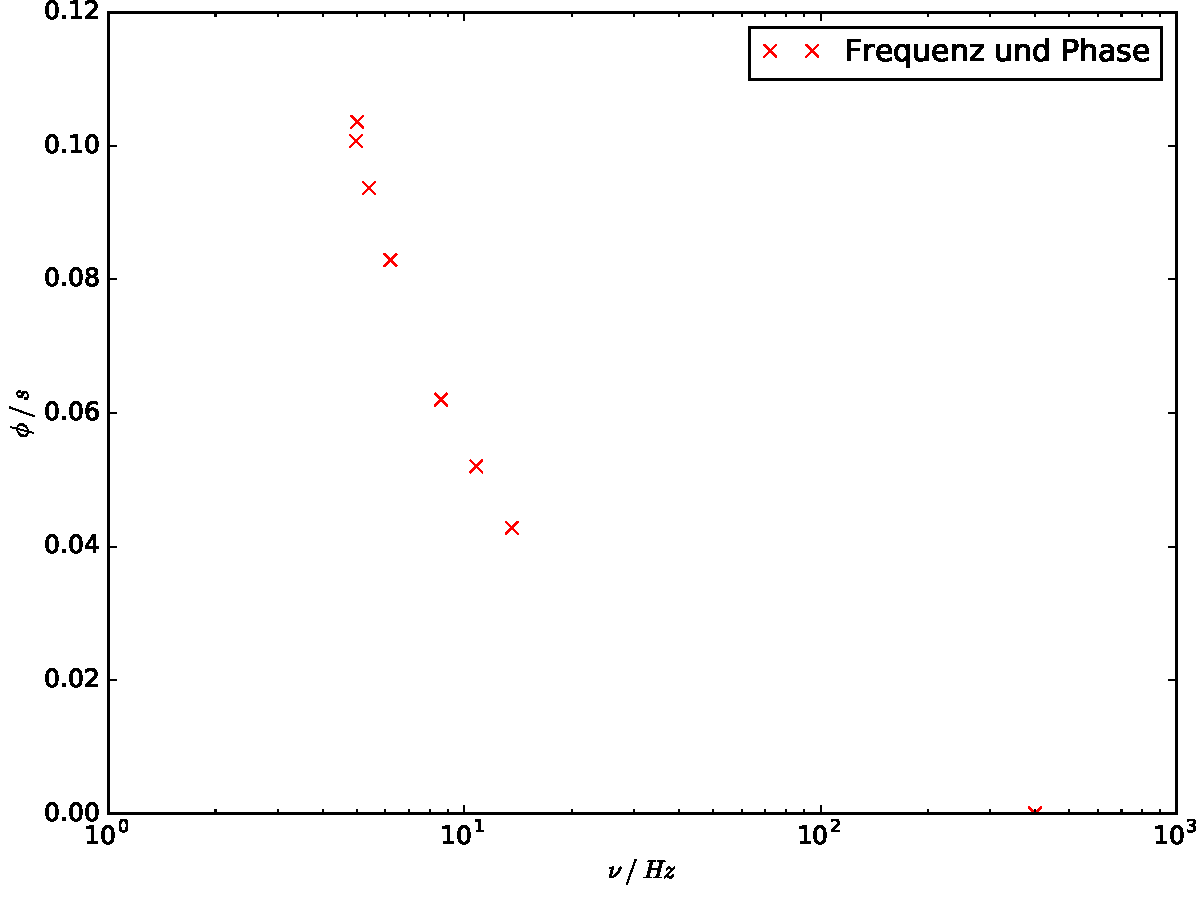
\includegraphics[height=7cm]{./logos/5dplot.pdf}
        \caption{Frequenzabhängigikeit der Phase zwischen Erreger-und Kondensatorspannung}
        \label{fig:5dplot}
      \end{figure}

    Die Messreihe ist in Taballe \ref{tab:5dtab} dargestellt.
    \begin{table}
      \centering
      \caption{Frequenzabhängigkeit der Phase zwischen Erreger-und Kondensatorspannung}
      \label{tab:5dtab}
      \sisetup{round-mode = places , round-precision = 2}
    \begin{tabular}{S S}
      \toprule
      $\nu/\symup{Hz}$ &  $\frac{\phi}{\symup{\mu s}}$ \\
      \midrule
      1.007000000000000000e+05 & 4.959999999999999964e+00\\
      2.323000000000000000e+03 & 0.000000000000000000e+00\\
      4.282000000000000000e+04 & 1.359999999999999964e+01\\
      5.200000000000000000e+04 & 1.080000000000000071e+01\\
      6.200000000000000000e+04 & 8.599999999999999645e+00\\
      8.290000000000000000e+04 & 6.200000000000000178e+00\\
      9.370000000000000000e+04 & 5.400000000000000355e+00\\
      1.036000000000000000e+05 & 5.000000000000000000e+00\\
      4.156000000000000227e+01 & 4.000000000000000000e+02\\
      5.500000000000000000e+01 & 4.000000000000000000e+02\\
      5.008000000000000114e+02 & 0.000000000000000000e+00\\
      1.985000000000000000e+02 & 0.000000000000000000e+00\\
      \bottomrule
    \end{tabular}
    \end{table}
    \FloatBarrier
    \subsection{Frequenzabhängigkeit des Scheinwiederstandes eines Serienkreises}
    \begin{figure}
      \centering
      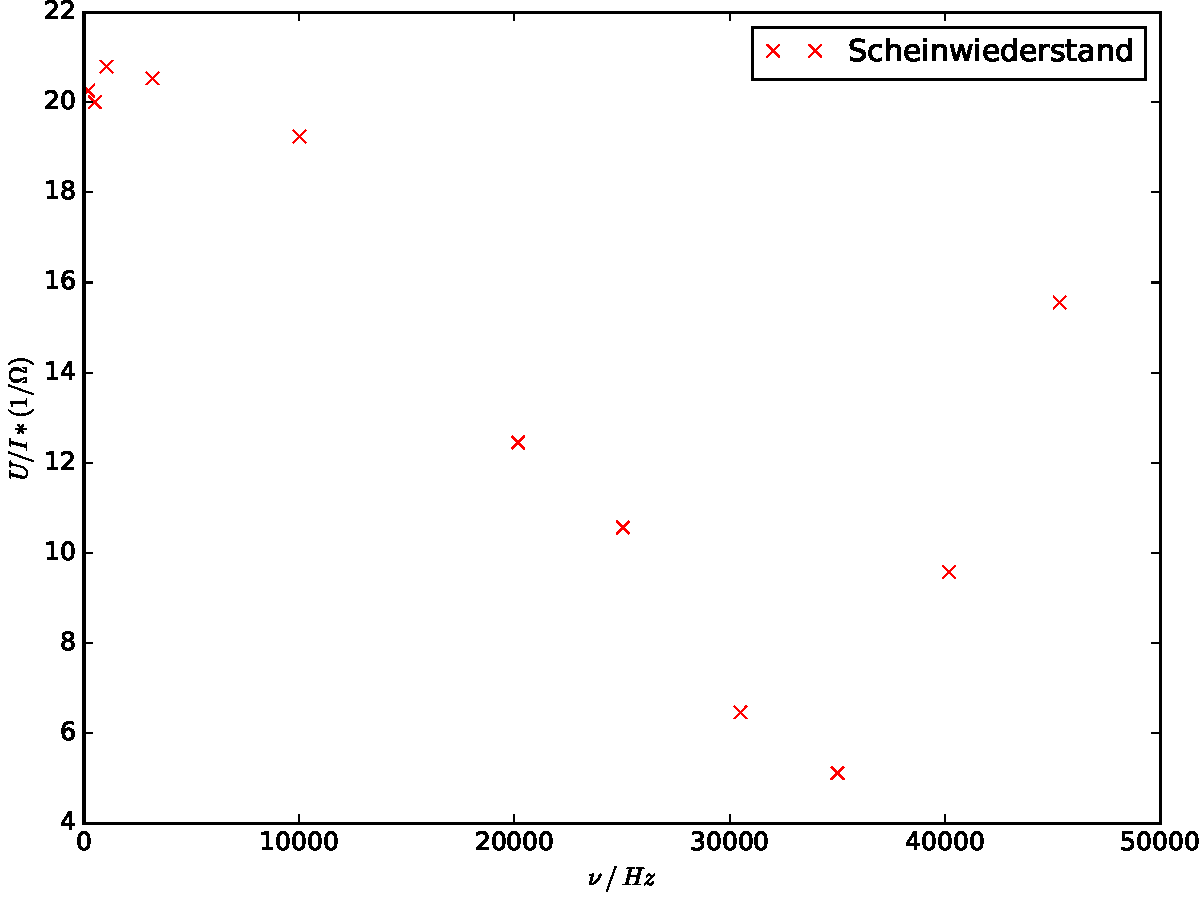
\includegraphics[height = 7cm ]{./logos/5eplot.pdf}
        \caption{Frequenzabhängigkeit des Scheinwiederstandes eines Serienkreises}
        \label{fig:5eplot}
      \end{figure}
      \FloatBarrier
      Der Plot \ref{fig:5eplot} zeigt den Abfall des Scheinwiederstandes bei
      steigender Frequenz. Jedoch steigt dieser
      wieder, dies steht im Wiederspruch zu unseren Erwartungen.
      Die Messreihe ist in der Tabelle \ref{tab:5etab} dargestellt.
\begin{table}
  \centering
  \caption{Frequenzabhängigkeit des Scheinwiederstandes}
  \label{tab:5etab}
  \sisetup{round-mode = places , round-precision = 2}
\begin{tabular}{S S S}
  \toprule
  $U_{pp}/\symup{V}$ & $ I_{pp}/\symup{A}$ &  $\nu/\symup{Hz}$ \\
  \midrule
  3.119999999999999929e+01 & 1.540000000000000036e+00 & 1.985000000000000000e+02\\
  3.119999999999999929e+01 & 1.560000000000000053e+00 & 5.108999999999999773e+02\\
  3.160000000000000142e+01 & 1.520000000000000018e+00 & 1.046000000000000000e+03\\
  3.080000000000000071e+01 & 1.500000000000000000e+00 & 3.185000000000000000e+03\\
  3.039999999999999858e+01 & 1.580000000000000071e+00 & 1.001000000000000000e+04\\
  3.000000000000000000e+01 & 2.410000000000000142e+00 & 2.017000000000000000e+04\\
  3.000000000000000000e+01 & 2.839999999999999858e+00 & 2.504000000000000000e+04\\
  2.919999999999999929e+01 & 4.519999999999999574e+00 & 3.050000000000000000e+04\\
  2.800000000000000000e+01 & 5.480000000000000426e+00 & 3.501000000000000000e+04\\
  2.919999999999999929e+01 & 3.049999999999999822e+00 & 4.019000000000000000e+04\\
  3.080000000000000071e+01 & 1.979999999999999982e+00 & 4.533000000000000000e+04\\
  \bottomrule
\end{tabular}
\end{table}
\FloatBarrier
